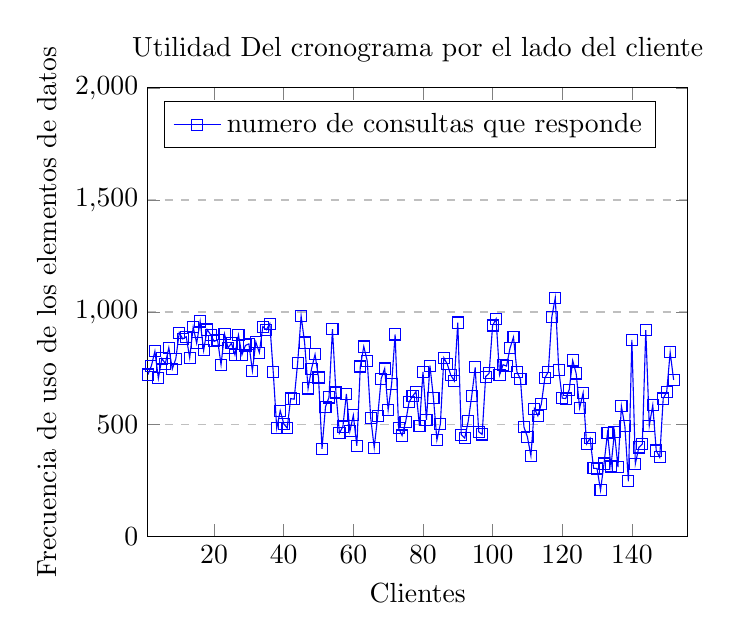
\begin{tikzpicture}
\begin{axis}[
    title={Utilidad Del cronograma por el lado del cliente},
    xlabel={Clientes},
    ylabel={Frecuencia de uso de los elementos de datos},
    xmin=1, xmax=156,
    ymin=0, ymax=2000,
    xtick={},
    ytick={},
    legend pos=north west,
    ymajorgrids=true,
    grid style=dashed,
]

\addplot[
    color=blue,
    mark=square,
    ]
    coordinates {
    %USO EXACTO
    (1,721)
(2,760)
(3,825)
(4,704)
(5,793)
(6,770)
(7,841)
(8,746)
(9,791)
(10,908)
(11,880)
(12,890)
(13,796)
(14,933)
(15,861)
(16,958)
(17,829)
(18,922)
(19,899)
(20,869)
(21,876)
(22,765)
(23,902)
(24,840)
(25,861)
(26,809)
(27,897)
(28,809)
(29,851)
(30,858)
(31,738)
(32,866)
(33,819)
(34,935)
(35,921)
(36,948)
(37,731)
(38,481)
(39,560)
(40,502)
(41,482)
(42,614)
(43,611)
(44,772)
(45,982)
(46,864)
(47,659)
(48,747)
(49,811)
(50,708)
(51,390)
(52,577)
(53,619)
(54,924)
(55,641)
(56,460)
(57,489)
(58,635)
(59,468)
(60,539)
(61,403)
(62,757)
(63,846)
(64,781)
(65,526)
(66,395)
(67,535)
(68,703)
(69,748)
(70,563)
(71,679)
(72,900)
(73,483)
(74,449)
(75,508)
(76,598)
(77,624)
(78,645)
(79,492)
(80,733)
(81,519)
(82,761)
(83,618)
(84,429)
(85,501)
(86,796)
(87,767)
(88,718)
(89,693)
(90,953)
(91,453)
(92,438)
(93,513)
(94,625)
(95,753)
(96,466)
(97,454)
(98,712)
(99,727)
(100,940)
(101,969)
(102,719)
(103,765)
(104,759)
(105,839)
(106,888)
(107,733)
(108,700)
(109,487)
(110,443)
(111,359)
(112,569)
(113,537)
(114,590)
(115,705)
(116,734)
(117,977)
(118,1064)
(119,742)
(120,616)
(121,614)
(122,653)
(123,784)
(124,726)
(125,572)
(126,639)
(127,412)
(128,437)
(129,303)
(130,302)
(131,205)
(132,324)
(133,460)
(134,311)
(135,464)
(136,308)
(137,580)
(138,490)
(139,245)
(140,876)
(141,323)
(142,396)
(143,411)
(144,919)
(145,493)
(146,584)
(147,382)
(148,352)
(149,614)
(150,643)
(151,820)
(152,697)
    };
    \legend{numero de consultas que responde}

\end{axis}
\end{tikzpicture}

